\clearpage
\chapter{Experimentations, Réalisations}
\label{sec:SOTA}

\section{Représentation Graphe/Squelette porteuse de sens}

\subsection{Introduction}
Le format de structure de données de la majorité des articulations disponibles via les approches de squelettisation en un tenseur ignore les relations de dépendance physique entre les articulations et ajoute de fausses connexions entre les articulations du corps qui ne sont pas liées physiquement.

\begin{figure}[H]
    \centering
    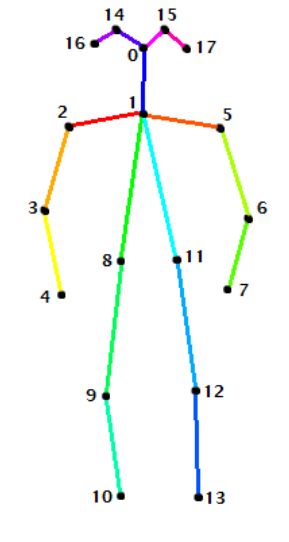
\includegraphics[width=0.3\linewidth]{Images/openpose.png}
    \caption{Structure de données de la représentation squelette obtenue à l'aide de la bibliothèque OpenPose \cite{cao2017realtime}}
    \label{fig:openPoseSkel}
\end{figure}

La figure \ref{fig:openPoseSkel}, nous permet de constater que conserver le squelette obtenu par les algorithmes de detection de pose classiques, sans avoir recours à une transformation pourrait réduire la qualité de nos résultats: certains couples d'articulations, bien que se suivant de manière incrémentale dans la structure de données utilisée, n'ont en réalité aucune raison valable de l'être: par exemple, l'extrémité gauche du bras et l'épaule droite (\textit{nodes 4 et 5}) ou encore l'extrémité droite du bras et la hanche gauche (\textit{nodes 7 et 8}).

Une grande majorité des travaux actuels semblent négliger l'importance de cette représentation spatiale et ne se focalisent que sur le coté temporel: la dynamique des articulations, sans remettre en question la structure de données spatio-temporelle en entrée.

\subsection{Méthodologie}

En reprenant les travaux de \cite{liu2016spatio} et \cite{2018arXiv180110304Y}, j'ai souhaité m'intérésser à cette question de représentation: en réalisant un Depth-First Search (DFS) sur un hub du graphe représentant le squelette. De cette manière, il est possible d'obtenir une structure de type arbre/graphe n'exploitant que des liens de voisinage entre joints existants.

\algnewcommand\algorithmicforeach{\textbf{for each}}
\algdef{S}[FOR]{ForEach}[1]{\algorithmicforeach\ #1\ \algorithmicdo}

\begin{algorithm}
 \caption{Explorer}\label{algorithm1}
 \KwIn{graphe G, sommet s}
  marquer le sommet s\;
  afficher(s)\;
 \ForEach {sommet $t$ fils de $s$}{
  \eIf{$t$ n'est pas marqué}{
    Explorer(G,t)\;
  }
 }
\end{algorithm}


\begin{algorithm}
 \caption{Depth-First Search (DFS)}\label{algorithm1}
 \KwIn{graphe G}
 %\KwOut{how to write algorithm with \LaTeX2e }
 %initialization\;
 \ForEach {sommet $s \in \mathcal G $}{
  \eIf{s n'est pas marqué}{
    explorer(G,s)\;
  }
 }
\end{algorithm}

L'exploration d'un DFS depuis un sommet $s$ fonctionne comme suit. L'algorithme poursuit  un chemin dans le graphe jusqu'à une feuille ou jusqu'à atteindre un sommet déjà visité. L'algorithme revient alors sur le dernier sommet où il était possible de suivre un autre chemin puis continue d'explorer. L'exploration s'arrête quand tous les sommets depuis $s$ ont été visités.

Ainsi, en reprenant la structure de données format tenseur d'un jeu de données, il est possible de réaliser un DFS afin d'obtenir une représentation respectant les relations de dépendance physique du squelette (\ref{fig:DFS}).

\begin{figure}[H]
    \centering
    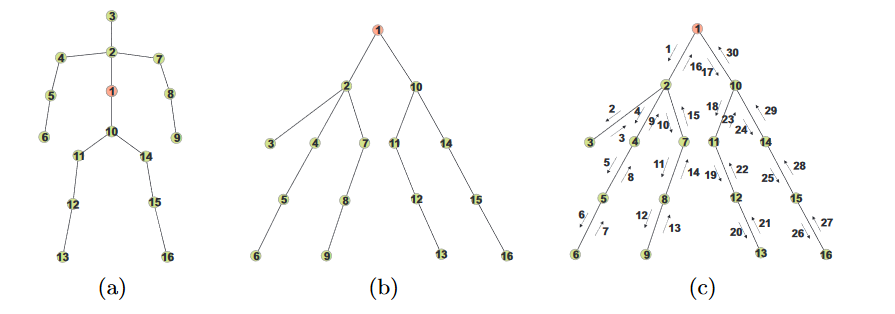
\includegraphics[width=1\linewidth]{Images/DFS.png}
    \caption{(a) Articulations du squelette d'un corps humain avec la structure de données initiale. L'ordre de visite des noeuds est incrémentale:1-2-3-...-16. (b) Le squelette est transformé en une structure arborescente. (c)  L'arbre peut être dépilé en une chaîne dont l'ordre de visite des noeuds conserve la relation physique des articulations: 1-2-3-2-4-5-6-5-4-2-7-8-9-8-7-2-1-10-11-12-13-12-11-10-14-15-16-15-14-10-1, Figure équivalente à la figure 2 dans  \cite{liu2016spatio}.}
    \label{fig:DFS}
\end{figure}

Souhaitant m'intéresser à la plus value apportée par cette représentation proposée par \cite{liu2016spatio} et \cite{2018arXiv180110304Y} pour la classification d'actions squelettiques, j'ai souhaité me comparer à un modèle de classification existant pour les mêmes conditions experimentales dans le cadre de convolutions 1D et convolutions 2D. Je me suis donc basé sur l'approche experimentale de Double-feature Double-motion Network \cite{2019arXiv190709658Y} ainsi que sur leur architecture présentée en \ref{fig:DDnet} pour les CNN 1D et avec un simple modèle convolutifs pour les convolutions 2D.


\begin{figure}[H]
    \centering
    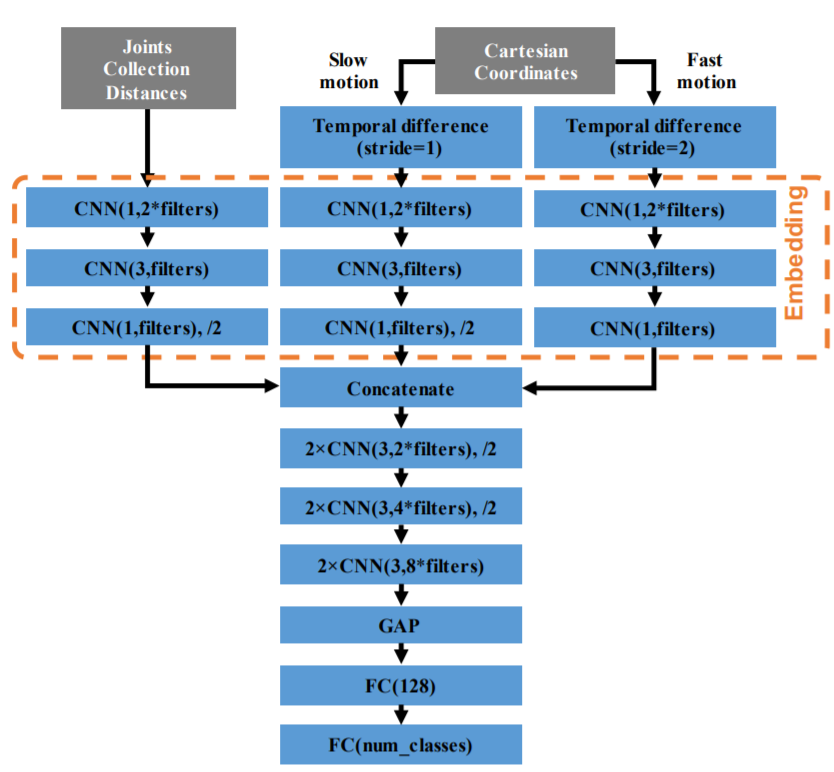
\includegraphics[width=0.55\linewidth]{Images/ddnet.png}
    \caption{L'architecture du réseau DD-Net. \textit{2×CNN(3,
2*filters),/2} désigne deux couches 1D ConvNet (taille du noyau
= 3, channels = 2*filtres) et un Maxpooling (strides = 2).GAP
désigne le Global Average Pooling. FC signifie "Fully Connected". La taille du modèle est ajustable en fonction de la variable \textit{filters}.}
    \label{fig:DDnet}
\end{figure}

\subsection{Tests et évaluations}
\subsubsection{Evaluation datasets et protocole d'évaluation}
Nous avons expérimenté les capacités de cette représentation sur deux jeux de données de reconnaissances d'action squelettiques: SHREC (actions de la main en 3D) proposé par \cite{de2017shrec} et JHMDB (action du corps en 2D)  proposé par \cite{jhuang2013towards}.\\

Simlairement à \cite{2019arXiv190709658Y} mais par manque de temps, SHREC est évalué pour un des deux cas : pour 14 gestes. L'ensemble de données JHMDB est évalué en utilisant des squelettes annotés manuellement, et l'évaluation se fait par cross-validation sur un split 3.

\subsubsection{Détails d'implémentation}
\subsubsection{Modèle CNN 1D}
L'entrainement se réalise sur une RTX 2080 Ti, les conditions experimentales ne diffèrent pas de \cite{2019arXiv190709658Y}.

\subsubsection{Modèle CNN 2D}


\subsubsection{Résultats et discussion}


\begin{table}[H]
\centering
\scalebox{0.95}{
\begin{tabular}{l|l|l|l} 
\hline
\textbf{Méthode}               & \textbf{Paramètres} & \textbf{14 classes} & \textbf{28 classes}  \\ 
\hline
DD-NET (64 filtres)     & 1.82M               & 94.6\%              & 91.9\%               \\
DD-NET (32 filtres)     & 0.50M               & 93.5\%              & 90.4\%               \\
DD-NET (16 filtres)     & 0.15M               & 91.8\%              & 90.0\%               \\ 
\hline
DFS-DD-NET (64 filtres) & 1.84M               & 95.9\%              &                      \\
DFS-DD-NET (32 filtres) & 0.51M               & 94.7\%              &                      \\
DFS-DD-NET (16 filtres) & 0.16M               & 93.1\%              &                     
\end{tabular}
}
\caption{Résulats obtenus grâce à la normalisation DFS sur SHREC \cite{de2017shrec} (Squelettes de main 3D)}
\end{table}

\begin{table}[H]
\centering
\scalebox{0.85}{
\begin{tabular}{l|l|l}
\textbf{Méthode}       & \textbf{Paramètres} & \textbf{Resultats}  \\ 
\hline
Chained Net \cite{2017arXiv170400616Z}             & 17.5M           & 56.8\%              \\
EHPI \cite{ludl2019simple}                   & 1.22M           & 65.5\%              \\
POTION    \cite{choutas2018potion}              & 4.87            & 67.9\%              \\
DD-Net (filters 64)     & 1.82M           & 77.2\%              \\
DD-Net (filters 32)     & 0.5M            & 73.7\%              \\
DD-Net (filters 16)     & 0.15M           & 65.7\%              \\ 
\hline
DFS-DD-NET (filters 64) & M               & \%                  \\
DFS-DD-NET (filters 32) & M               & \%                  \\
DFS-DD-NET (filters 16) & 0.15M           & 66.4\%                 
\end{tabular}}
\caption{Résulats obtenus grâce à la normalisation DFS en conservant l'architecture  \cite{2019arXiv190709658Y} sur JHMDB \cite{jhuang2013towards} (Squelettes corps humain 2D)}
\end{table}



\section{Autoencodeur semi-supervisé pour l'action recognition}

\subsection{Introduction}
Les auto encodeurs étant une composition de transformation non linéaires en esperant trouver une représentation dans l'espace adaptée au format des données et conservant un maximum de sémantique de celui-ci.

Je me suis intéréssé à cette question de représentation pour plusieurs raisons:
\begin{itemize}
    \item Tout est une question d'embedding et de normalisation en machine learning. Au final, le role premier des couches cachées est de transformer cet embedding en espérant qu'il soit porteur d'information. Le jour où l'on trouve un moyen de normaliser et de représenter les données de manière plus adequate, n'importe quel classifieur pourra obtenir de bons résultats pour peu que les données d'entrée soient porteuses d'information. Le jour ou l'on arrivera à obtenir une représentation utilisable plus rapidement au lieu de stacker des layers au sein d'un réseau de neurones, d'autres problématiques d'apprentissage apparaitront mais le gain serait intéréssant: (Selon le théorème d'approximation universelle, n'importe quel Shallow Network peut supposément approximer une fonction donnée \cite{universalapproxtheorm,scarselli1998universal}).
    
    \item En s'intéréssant à la question de la représentation des données, on évite un apprentissage de cette représentation à "l'aveugle" (en optimisant un réseau précis sur un jeu de données précis et en testant un maximum d'hyperparamètres on est assurés de faire un bon résultat.  On peut potentiellement réduire la taille de notre réseau et donc par définition réduire le temps d'inférence de celui-ci, ce qui peut être intéréssant dans le cadre d'un sujet en temps réel.
\end{itemize}

L'idée étant d'entrainer un autoencodeur avec une fonction de coût modifiée en rajoutant une contrainte sur la séparation linéaire des classes dans l'espace latent (LDA / QDA / FDA). Il a été montré que la représentation optimale interne d'un MLP s'obtient en faisant une analogie avec une analyse discriminante non linéaire \cite{webb1990optimised}.

Les approches factorielles citées plus haut s'apparentent à la projection de données dans l'espace comme celle d'une ACP mais tandis que l'ACP maximise la variance du jeu de données, celles-ci se focalisent sur la maximisation de la séparabilité des classes dans l'espace (supervisé). On obtiendrait donc un AutoEncodeur "semi-supervisé" dans le sens où celui-ci se focalise sur deux informations complètement différentes dans les données, l'une de manière non-supervisée, l'autre de manière supervisée:
\begin{itemize}
    \item La structure inhérente des données capturée de manière non supervisée grâce à l'Auto-encodeur, on conserverait une partie de l'information importante et discriminante du jeu de données. (feature extraction)
    \item La séparabilité des classes dans l'espace grâce à l'analyse discriminante (non) linéaire. Ce qui permettrait de réduire le nombre de layer au final.
\end{itemize}{}


Une fois la convergence obtenue, on peut imaginer deux utilisations:
\begin{itemize}
    \item Récupérer cet espace latent combinant les informations "data driven" grâce à l'apprentissage non-supervisé de l'auto encodeur classique et une première ébauche de séparabilité linéaire grâce à la seconde partie de la fonction de coût. Envoyer l'espace latent à un input de CNN classique très peu profond, GAP, Softmax ou un MLP, Softmax. Finetuner le réseau de bout en bout et voir ce que cela donne quand à la capacité de discrimination de l'approche. 
    \item Générer des données en réalisant une génération d'instance au niveau de l'espace latent grâce à des approches type SMOTE \cite{chawla2002smote} ou ADASYN \cite{he2008adasyn}  et utiliser la partie décodeur pour  faire de la data génération.
\end{itemize}

\subsection{Formalisation}
On pose le problème comme ceci: \newline
$$\min _{\theta_{1}, \theta_{2}},\left\|\mathbf{X}-g_{\theta_{2}}\left(f_{\theta 1}(\mathbf{X})\right)\right\|^{2}$$

Fonction de coût habituelle d'un autoencodeur avec $\theta_{1}, \theta_{2}$ les paramètres des blocs encodeur et decodeur de l’AE. 

$$\min _{\theta_{1}, \theta_{2}, \mathbf{S}}\left\|\mathbf{X}-g_{\theta_{2}}\left(f_{\theta_{1}}(\mathbf{X})\right)\right\|^{2}+\lambda\left\|f_{\theta_{1}}(\mathbf{X})-\mathbf{S}_{f_{\theta 1}}(\mathbf{X})\right\|^{2}$$

Ajout d'une variation dans la fonction de coût: avec S la matrice de projection des individus dans l'espace latent obtenue avec une analyse discriminante linéaire (LDA) et $\lambda$ un régularisateur.

Une fois, l'entrainement de l'autoencodeur réalisé, récupération des poids de la partie encodeur: $f_{\theta 1}$, ajout d'une fonction classifieur softmax:\\ 

$\sigma(\mathbf{z})_{j}=\frac{\mathrm{e}^{z_{j}}}{\sum_{k=1}^{K} \mathrm{e}^{z_{k}}} \text { pour  tout } j \in\{1, \ldots, K\}$


\begin{figure}[H]
    \centering
    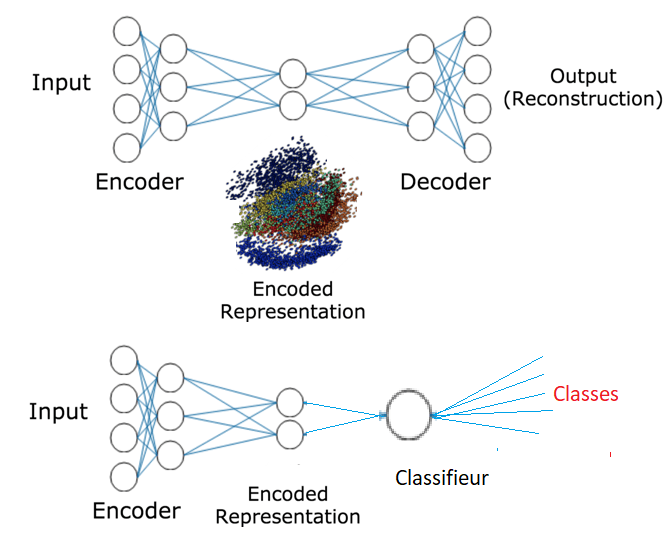
\includegraphics[width=0.8\linewidth]{Images/Autoencoder_modif.png}
    \caption{Pipeline de l'approche}
    \label{fig:AEmodif}
\end{figure}

\subsection{Tests et évaluation}
J'ai réalisé l'implémentation de cette approche sur deux jeux de données: SHREC \cite{de2017shrec} et JHMDB \cite{jhuang2013towards}.\\

\begin{table}[H]
\centering
\scalebox{0.75}{
\begin{tabular}{l|l|l|l|l}
\hline
\textbf{Méthode}                                 & \textbf{Nb Params} & \textbf{SHREC 14} & \textbf{SHREC 28} & \textbf{FPS (RTX 2080 ti)}  \\ 
\hline
LDA sur l'input                   &          - &         33.0\% &          27.6\%&      \\
LDA sur le bottleneck AE classique (\lambda = 0)              &          - &         37.9\% &          42.8\%&      \\
LDA sur le bottleneck AE modifié (\lambda = 5)              &          - &         43.5\% &          35.6\%&      \\
\hline
MLP Sans initialisation                      &          1.2M &         91.2\% &          85.2\%&     20 000 \\
MLP Avec initialisation AE classique (\lambda = 0)        &          1.2M &          91.5\%&          85.9\%&      -\\
MLP Avec initialisation AE Modifié (\lambda =1) &          1.2M &          91.9\%&          87.6\%&      -\\
MLP Avec initialisation AE Modifié (\lambda = 2.5) &           1.2M&          92.4\%&          86.9\%&     -\\
MLP Avec initialisation AE Modifié (\lambda = 5)          &          1.2M &          \textbf{92.5\%}&         \textbf{87.1}\% &      -\\
MLP Avec initialisation AE Modifié (\lambda = 7.5) &          1.2M &         91.9\% &          86.4\%&      -\\
MLP Avec initialisation AE Modifié (\lambda = 10) &          1.2M &          90.9\%&          85.2\%&      -


\end{tabular}}
\caption{Résulats obtenus grâce à l'initialisation des poids avec un AE modifié sur SHREC \cite{de2017shrec}}
\end{table}




\begin{table}
\scalebox{0.7}{
\centering
\begin{tabular}{l|l|l|l} 
\hline
\textbf{Methode}                  & \textbf{Nb Params} & \textbf{\textcolor[rgb]{0.129,0.145,0.161}{Average accuracy of 3 splits ~})\textcolor[rgb]{0.129,0.145,0.161}{}~} & \textbf{Classifications par secondes}  \\
\hline
Chained Net (ICCV17)              & 17.50 M            & 56.8\%                                                                                                                                        & 33 (1080 Ti)                           \\
EHPI~ (ITSC19)                    & 1.22 M             & 65.5\%                                                                                                                                        & 29 (1080 Ti)                           \\
PoTion (CVPR18)                   & 4.87 M             & 67.9\%                                                                                                                                        & 100 (1080 Ti)                          \\
DD-Net                            & 1.82M              & 77.2\%                                                                                                                                        & 2,200 (1080 Ti)                        \\ 
\hline
Sans initialisation (\lambda =0)~ & 0.67M                  &   65.2\%                                                                                                                                            & -                                      \\

Avec initialisation AE classique (\lambda =0)~ & 0.67M                  &   66.4\%                                                                                                                                            & -                                      \\
Avec initialisation AE modifié (\lambda =1)    & -                  &          66.2\%                                                                                                                                     & -                                      \\
Avec initialisation AE modifié (\lambda =2.5)   & -                  &          68.3\%                                                                                                                                     & -                                      \\
Avec initialisation AE modifié (\lambda =5)   & -                  &        67.9\%                                                                                                                                       & -                                      \\
Avec initialisation AE modifié (\lambda =7.5)   & -                  &          66.5\%                                                                                                                                     & -                                      \\
\hline
\end{tabular}}
\end{table}

\begin{figure}[H]
    \centering
    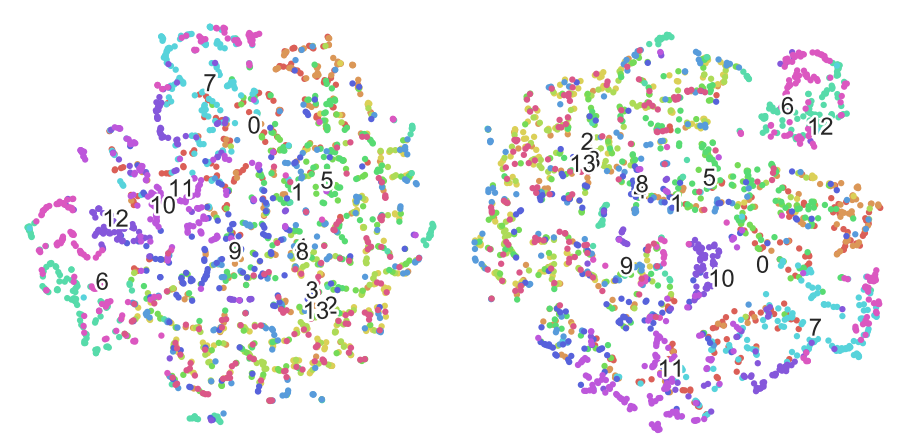
\includegraphics[width=0.8\linewidth]{Images/tsne_results.png}
    \caption{Visualisation des espaces latents via T-Sne: à gauche auto-encodeur classique, à droite auto-encodeur modifié ($\lambda$ = 10)}
    \label{fig:AEmodifTSNE}
\end{figure}

\begin{figure}[H]
    \centering
    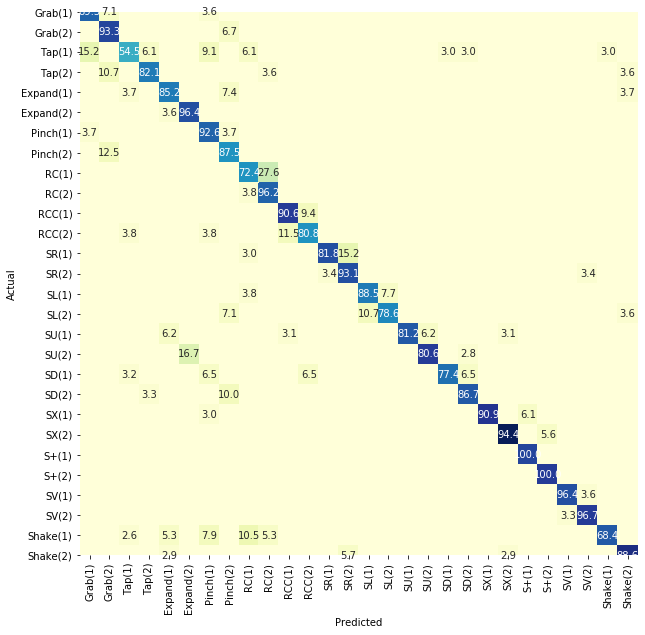
\includegraphics[width=0.8\linewidth]{Images/shrec28.png}
    \caption{ca}
    \label{fig:rsshrec28}
\end{figure}\textbf{}

\subsection{Remarques}
\begin{itemize}
    \item Le nombre maximum d'axes obtenus par la LDA correspond au nombre de classe moins un: sur SHREC 14 l'espace latent est donc de dimension 13 toute représentation avec un espace latent superieur est impossible (on ne peut donc difficilement imposer des contraintes de sparsité au modèle). Cela implique également une perte très lourde de l'information vis-à-vis de l'information dans l'espace latent. (SHREC: de 2122 neurones d'entrée à un espace latent avec 13 neurones)
    \item Quelques problèmes de convergence dûs à l'optimisation de $\lambda$ durant l'apprentissage de l'autoencodeur avec la fonction de coût modifiée(optimiser ADAM \cite{kingma2014adam}).
\end{itemize}

\subsection{A creuser}

Essayer plusieurs structures plus travaillées qu'un simple MLP:
\begin{itemize}
    \item AE: Convolutions / Attention / Séquentiel / VAE.
    \item analyse discriminante: QDA  pour ne pas émettre de suppositions vis-à-vis des matrices de covariance de chaque classes
\end{itemize}

Rien n'est fixé dans la fonction de coût, j'imagine qu'ajouter un autre critère de régularization ne peut être que bénéfique, mais vu les prolèmes de convergence actuels, je préfère ne pas le tenter pour l'instant.


